\documentclass[./main.tex]{subfiles}

\begin{document}

\chapter{Introduction}\label{chapter:introduction}

% Citation
"Only what is evolving is alive" \footnote{Pierre Kerner translation from french, original quote "N'est vivant que ce qui évolue"} this definition of life, like many others, is incomplete and we can probably find some corner case. This definition is based on the definition of evolution, we can try to define evolution of a thing, as the change on the thing to optimize her capability to conserve her self. To do that a thing need a memory.

In majority of actual know life form store this memory in DNA for DeoxyriboNucleic Acid. DNA is a molecule compose by two strain, each strain was composed by phosphate backbone, along of these backbone we have sugar linked to a nucleic acid. We have four type on nucleic acid: Adenine (A), Thymine (T), Cytosine (C) and Guanine (G), Figure \ref{intro:fig:dna_rna_pres} show 3d structure of DNA.

The two strands of DNA are linked by their nucleic acid, with some rules in front of an A we will always have a T in front of a C we will always have a G and vice versa, a DNA strain was a complementary of the other. But we cannot add a new DNA base to each DNA strain at the same end, for some of chemical properties that we will not detail here, we say DNA was composed by two anti-parallel strain. If we want know the composition of the other DNA strain for another one we need to made two operation complementary (replace A by T, T by A, C by G and G by C) and reverse the order. 

In bioinformatics we generally represent a DNA strain by string in a four letter alphabet (A, C, T, G) and we can get the other strain by reverse complement operation.

\begin{figure}[ht]
    \centering
    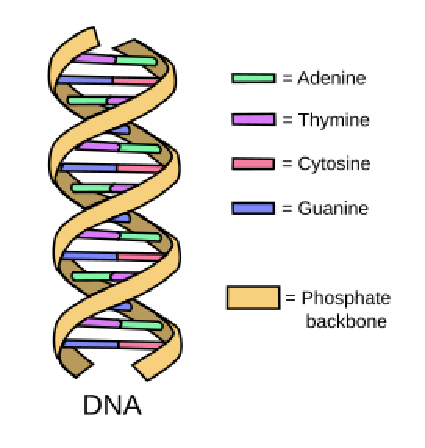
\includegraphics[]{introduction/images/DNA.pdf}
    \caption{Structure and composition of DNA Source: Wikipedia \protect\url{https://en.wikipedia.org/wiki/File:DNA_simple2.svg}}
    \label{intro:fig:dna_rna_pres}
\end{figure}

With mainy complexe and not details her, information contains in DNA was used to build essential molecules that keep the organism alive, reproduce it. This information is therefore the basis of the organism's functioning, if this information is destroyed or modified, the living organism will behave differently or died. So knowing and understanding the succession of DNA bases and therefore an effective entry point for analyzing many biological phenomena, disease, speciation event,…

To read this information we have many biochemical techniques that we group under the term Sequencing these techniques will allow us to read fractions of DNA fragments more or less long and with a variable error rate.

\section{Sequencing}

Sequencing technology evolve quickly since 1977\cite{sanger_sequencing}, even if it is an a posteriori reconstruction, three generations can be distinguished, based on reads property. In this section we didn't detail the biochemic methods we just focus on reads property and her impact on different bioinformatics task.

The two most important properties of a read are its size and error rate\. The longer of a read provide more information about his original sequence, which facilitate downstream analysis. If read contains many errors, the cost of downstream analysis increase and lost in precision and recall.

Sanger technique create large reads with very small error rate, but with a very low throughput and very expensive cost per base.
Second generation increase the throutput and reduce the cost per base, by reducing the length of the reads and increasing the probability of error ($\approx$ 1\%). This type of error are most of the time a substitution between two nucleotides, sequencer read \texttt{A} in place of a \texttt{T}.
The third generation has greatly increased the size of the reads but also the error rate while maintaining a descent throughput. Error in third generation are mostly insertion deletion, sequencer didn't read a part of sequence or generate random base not present in original sequence. Table \ref{intro:tab:technology_property} present read length and error rate on many technology.

\begin{table}[ht]
    \centering
    \begin{tabular}{l|rr|l}
         Technology          & Read length (bd)                 & Error rate    & Source                          \\ \hline
         ABI/Solid           & 75                               & Low ($\approx$ 2\%)    & \cite{seq_assembly_demystified} \\
         Illumina/Solexa     & 100–150                          & Low (<2\%)             & \cite{seq_assembly_demystified} \\
         IonTorrent          & $\approx$ 200                    & Medium ($\approx$ 4\%) & \cite{seq_assembly_demystified} \\
         Roche/454           & 400–600                          & Medium ($\approx$ 4\%) & \cite{seq_assembly_demystified} \\
         Sanger              & $\approx$ 2 kb                   & Low ($\approx$ 2\%)    & \cite{seq_assembly_demystified} \\
         Pacific Biosciences & $\approx$ 10 kb ($\max$ 100 kb)  & High ($\approx$ 18\%)  & \cite{seq_assembly_demystified} \cite{longread_dark_matter} \\
         Oxford Nanopore     & $\approx$ 10 kb ($\max$ 1 mb)    & High ($\approx$ 12\%)  & \cite{longread_dark_matter} \cite{nanopore_read_accuracy} \\
    \end{tabular}
    \caption{This table present length of reads and error rate of main sequencing technology. Pacific Biosciences and Oxford Nanopore evolve quickly and this value change we have tried to be as up-to-date as possible but between two publications these values vary considerably.}
    \label{intro:tab:technology_property}
\end{table}


DNA sequencing was very useful tools for many analysis, and in some cases is mandatory to be able to understand biological mechanisms. In this thesis we while focus only on genome assembly problem it's a important usage of sequencing but the only one.

\section{Assembly algorithm}

If you want study an organism, knowing the complete genome sequence is very useful for a lot of task like find the genes or the sequence variations across a population. Yet, the best sequencing technologies still provide reads that are at least 2 orders of magnitude shorter than the genome. To understand the assembly problem, we provide a useful analogy which, to the best of our knowledge, has never been formulated before.

Imagine a crazy copyist monk. He is copying a book but he randomly chooses where he starts to copy, and he only copies small fragments of text at a time.
The copyist monks make errors, e.g. he would sometimes replaces a symbol by another one, would skip a symbol, or would add a random symbol. We respectively call these errors substitutions, deletions and insertions.
Now imagine that there are multiple such copyist monks.
They choose randomly where they begin to write. They can choose several times the same region of the book, never choose to copy a certain region, or more rarely copy another region. We refer by "coverage" the number of times a given chunk of the original book is copied. Coverage may significantly differ from one region to another.
In this analogy, the book is the genome of the organism we want to study, and the copyist monks are our sequencer. The fragments of text are reads, and the operation to rebuild the book is assembly.

The assembly task can be summary has a order problem we try to put the text fragments in the right order. \rc{Pas compris cette phrase}\pim{c'est mieux ?}

To find the right order of book fragments, we can try to compare fragments and say that e.g. this fragment is the same of this one, or these two fragments share the same symbols at their extremities. When two reads share a common sequence at their at the end of the reads we say they overlap \ref{intro:fig:overlap:perfect}. Yet it possible for reads to share a common sequence just because alphabet have a fixed size, but the probability of this event decrease when the length of common sequence increase. Intuitively, this probability gets smaller as overlaps get longer. In perfect word, the only criteria to evaluate whether an overlap is "real" or not should be the length of the overlap, the only criteria to evaluate if an overlap is a true one should be his length. However the number of errors in each reads broke this paradigm and force us to build  yet an important factor do consider is that reads contain errors \ref{intro:fig:overlap:erroneous}.

To reconstruct the original sequence with short fragments (reads), finding the overlaps between these fragments constitutes the basis of many assembly algorithms.

\begin{figure}[ht]
    \centering
    \subfloat[ht][$R_1$ share 7 bases at its end with the beginning of $R_2$, without any error]{
        \subfile{introduction/tikz/perfect_overlap.tex}
        \label{intro:fig:overlap:perfect}
    }
    \subfloat[ht][$R_1$ share 5 bases at its end with $R_3$, with one substitution and one deletion]{
        \subfile{introduction/tikz/erroneous_overlap.tex}
        \label{intro:fig:overlap:erroneous}
    }
    \caption{When reads didn't contains error all overlap look like (a) but}
    \label{intro:fig:overlap}
\end{figure}

\subsection{How to find overlap}

Find overlap between reads are generally the bootleneck of many assembly algorithm. 
This is a complete research field with many tools, \citeauthor{ovl_bench} produce a interesting benchmark about some of them. We details how of \mhap and \minimap works in section \ref{subsubsec:sota:canu} and \ref{subsubsec:sota:miniasm}.

\pim{sa n'a peut-être pas sa place ici} \rc{C'est pas mal de le mentionner. Tu peux juste dire ici que c'est un domaine de recherche à part entiere et citer quelque papiers. Et faire un rapide apercu des techniques utilisées (mentionner LCP, etc)}

\subsection{\textit{Greedy} assembly algorithm}

\pim{rajouté des citations}
The \textbf{Greedy} assembly algorithm are the first type of assembly tools, used on Sanger data. Algorithm \ref{intro:algo:greedy} present global idea how \textbf{Greedy} algorithm work.

The LONGEST\_OVERLAP function is the main part of algorithm the best overlap is the larger one or the overlap with less error, each algorithm have her own choose method.

\begin{algorithm}[ht]
    \caption{A greedy assembly}
    \begin{algorithmic}[1]
    \Function{greedy}{reads}\Comment{reads is a set of read}
        \State choose r1 in reads
        \State sequence $\leftarrow$ r1
        \While{r2 $\leftarrow$ \Call{best\_overlap}{r1}}\Comment{\Call{best\_overlap}{\null} is a function for r1 they get read r2 the best overlap for read r1 in reads}
            \State \Call{concatenate}{sequence, r2}
            \State \Call{drop}{r1, reads}
            \State r1 $\leftarrow$ r2
        \EndWhile
    \EndFunction
    \end{algorithmic}
    \label{intro:algo:greedy}
\end{algorithm}

Moreover \textbf{Greedy} algorithm, by focusing on the local problem, weach overlap is the best one for this read, can't manage repetition. Genome contains many repetition, like a book some word are reused or complete part of sentence can be present multiple time.

Figure \ref{intro:fig:greedy:repetition} present a case where reads $R_0$ $R_1$ and $R_2$ contains a repetition. $R_0$ have two possible overlap if overlap with $R_1$ is choose the assembly sequence match with the green path, if overlap with $R_2$ is choose the assembly sequence match with the red path. We can't know weach path is the good one and we didn't see the repetition. So assembly tools based on \textbf{Greedy} algorithm can produce many misassembly. 

\begin{figure}[ht]
    \centering 
    \subfile{introduction/tikz/repetition.tex}
    \caption{Each black box are a read, the grey box mark the position of a repetition. The begin of $R_1$ and $R_2$ are in repetition they share same begin but didn't match at her end. This repetition create a ambiguity in assembly.}
    \label{intro:fig:greedy:repetition}
\end{figure}

\subsection{Overlap Graph Consensus}

To solve trouble of repetition in \textit{Greedy} algorithm, \pim{ref necessaire} define an Overlap Graph Consensus (\OLC). Each read was a node and we build a edge between node if reads share an overlap. Figure \ref{intro:fig:olc:graph}, present the \OLC corresponding to ovelap present in \ref{intro:fig:greedy:repetition}.

We can see this graph like an ordering of piece of book provide by crazy monky, an edge indicate this piece of text was before this piece of text in the original book.

The repetition create a fork in \OLC, a node with two successor, it's easy to detect this case in graph and stop assembly. The result of assembly of this graph was 3 sequences with white node, green node and red node. The assembly was more fragmented than \textit{Greedy} algorithme but the assembly didn't contains misassembly.

\begin{figure}[ht]
    \centering 
    \subfile{introduction/tikz/overlap_graph.tex}
    \caption{Each node are a read and an edge was build between two read if they share an overlap.}
    \label{intro:fig:olc:graph}
\end{figure}

\pim{peut-être pas sa place ici}
In Figure \ref{intro:fig:olc:graph} you can notice edge from $R_1$ to read $R_3$, this overlap was exact we can found an overlap between $R_1$ and $R_3$. But this edge didn't provides a new information we know $R_1$ is before $R_3$, this edge was call a transitive edge. Gene Myers propose in \cite{string_graph} another assembly graph the string graph is an overlap graph without transitive edge.

If we have good string graph we just need follow simple path (path were all nodes have just one successor), to build assembly without misassembly.

\subsection{DeBruijn Graph}

A main trouble of \OLC strategy was the cost to find overlap between reads. In \citeauthor{eulerian_approach} in \cite{eulerian_approach} propose a new approch to solve assembly problem, without search of overlap between reads.

This approch was based on DeBruijn Graph (or \DBG), for an alphabet with $n$ symbol a \DBG represent each word of length $k$ as node and build a directed edges if node share $k - 1$ symbol at extremity, for example in Figure \ref{intro:fig:dbg:graph} node \texttt{ATCG} and \texttt{TCGG} share \texttt{TCG}. A word of length $k$ was called a \kmer.

In assembly problem $n = 4$ (${A, C, T, G}$), and we can choose a value of k between 1 and the length of read. In practice this size is often smaller than the size of a reads is the choice of the right values of k, depending on the use that we will have of the \DBG graph could be the subject of a completed thesis.

To build the \DBG we choose a value of $k$ and we add all \kmer present in reads in the \DBG. The \DBG used in assembly contains only \kmer present in dataset not all possible \kmer, and edge can be only edge present in dataset or all possible edges.

\begin{figure}[ht]
    \subfile{introduction/tikz/debruijn_graph.tex}
    \caption{The \DBG build for sequence \texttt{ATCGGATTCGCGGTGGTTTCG}. Each node was a word and if a word share $k - 1$ symbol at is end with $k - 1$ symbol at begin of another node we build a directed edge. This \DBG contains cycle this cycle match with a repetition in original sequence}
    \label{intro:fig:dbg:graph}
\end{figure}

Like \OLC we can detect repetition by inspect the number of successor of a node Figure \ref{intro:fig:dbg:graph} present a \DBG with a repetition. After build the \DBG we can follow the simple path to rebuild the original sequence.

With \DBG strategy we didn't compute overlap between reads, but the length of word in graph was shorter. And all repetition with a size upper than $k$ create cycle in the graph and fragment the assembly.

Moreover the overlap between word in \DBG must exact (without error) and with a fixed length ($k - 1$), these two constraints are particularly problematic when the reads contain a lot of error or when the coverage of the region is low.

%\subsection{Hybrid assembly}

%\section{Sequencing technology}

%\subsection{First generation}

%\subsection{Second generation}

%\section{Correction}

\subsection{Graph cleaning}

\OLC and \DBG was based on graph, the meaning of nodes and edges are different in this top type of graph. But we can found same structure in them, bubbles and tips.

Figure \ref{intro:fig:cleaning}

\begin{figure}[ht]
    \subfloat[][A example of tips in an assembly graph, the tips node wase represent in read, green, blue and black line underline different possible assembly scenario]{
        \subfile{introduction/tikz/cleaning_tips.tex}
        \label{intro:fig:cleaning:tips}
    }
    \subfloat[][A example of bubble in an assembly graph, each path was colored in different color. The length of each path can be different and we can have more than two path in bubble]{
        \subfile{introduction/tikz/cleaning_bubble.tex}
        \label{intro:fig:cleaning:bubble}
    }
    \caption{}
    \label{intro:fig:cleaning}
\end{figure}

\paragraph{Tips}

A tips in an assembly graph is a node with only on edge, a tips can be create by many thing, trouble during DNA extraction, DNA duplication, sequencer create an artefact, a read with to many error ….

As we can see in Figure \ref{intro:fig:cleaning:tips} a tips can create a branching node in middle of simple path, if we keep this tips generaly assembly create two contigs one before tips and one after tips (green and blue assembly scenario). If we remove this tips we can run the black scenario.

Its easy to detect and remove tips in graph, in many assembly tools tips are considered as errors and are removed.

\paragraph{Bubble}

We can define a bubble as a set of subpath in graph with same parent and same children, Figure \ref{intro:fig:cleaning:bubble} present an example with two path with same length. The bubble can be create by repetition or heterozygotie one or more version of this sequence contains a substitution or more complexe mutation.

If bubble are large it can be harder to detect, with small bubble one version of the bubble are kept the choose of the version can be based on random choice or on coverage or other magic tricks.

\section{Why people use long reads}

The length of read have a huge impacte on assembly, 

\section{Assembly Trouble}

\subsection{Data management}

Sequencing generate more and more data, and long-read sequencing technology work how to increase the throughout of sequencer. Tools around long-read assembly generate more data (overlap, assembly graph, contigs, hétérozygotie), and many times all this data isn't useful for a specific downstream analysis \pim{est-ce que fournir une référence est necessaire}.

Moreover some long-reads contains very bad quality region \cite{blog_post_error_repartition}.

Can we filter overlapping information with a positive (or not very bad) impact on assembly result, to increase speed of assembly and the impacte of assembly step on disk space ?
Can we found very bad quality region in long-read and remove it before any other analysis to increase quality and computation time of downstream analysis ?

We try to answer to this two question in paper "\yacrd and \fpa: upstream tools for long-read genome assembly"

\subsection{Trouble with heuristic algorithm}

Assembly tools perform a greate job, but they can't explore all space.
Due to memory constraint and cpu usage you can't build and store all overlap.
Due to theoretical limit, how many of base need to be share between to read to create an overlap how many error we can accept in this overlap.

Assembly tools need use heuristic algorithm, solve assembly trouble in this constraint, in majority of case this heuristic perform a very good work, but in some case we need perform a more complex analysis.

We try to build tools to simplify analysis of assembly tools result and help user to make choice for improve assembly quality in paper "Graph analysis of fragmented long-read bacterial genome assemblies"

\onlyinsubfile{
\bibliographystyle{plainnat}
\bibliography{main}
\addcontentsline{toc}{chapter}{Bibliography}
}

\end{document}